%source mathadata
\begin{multicols}{2}
			\begin{MADenumerate}
				\item \textbf{Calcul de \(m\) :}
				$$m=\dfrac{y_B-y_A}{x_B-x_A} = \dfrac{3-2}{3-1} = \dfrac{1}{2} = 0,5$$

				\item \textbf{Calcul de \(p\) :}

				Remplaçons par le point \(A(1,2)\) dans l'équation \(y=0,5 x+p\) :

				\(2=0,5\cdot 1 + p = 0,5 + p\).

				Donc \(p=2-0,5=1,5.\)

				\item  \(\boxed{\text{Équation finale : } y=0,5 x + 1,5.}\)

				\item Le coefficient directeur $m=\displaystyle\frac{1}{2}=0,5$ est cohérent avec le graphique : 2 unités à droite correspondent à 1 unité vers le haut.

				De même, par lecture graphique, l'ordonnée à l'origine $p$ est comprise entre 1 et 2 et semble bien au milieu de ces deux valeurs, donc $p=1,5$ est également cohérent.

				\begin{center}
					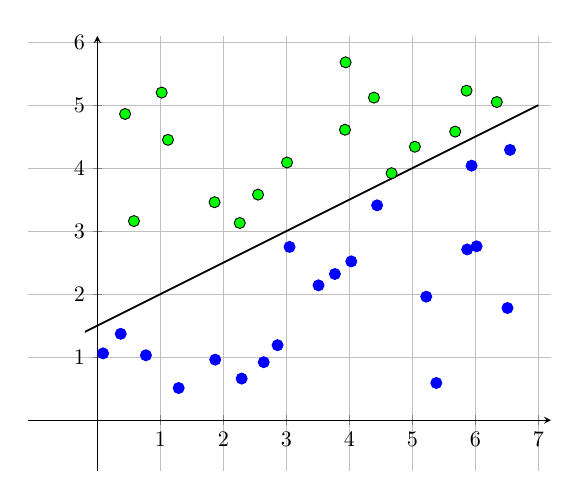
\begin{tikzpicture}[scale=0.8]
						\begin{axis}[
								x=1cm,y=1cm,
								axis lines=middle,
								ymajorgrids=true,
								xmajorgrids=true,
								xmin=-1.1,
								xmax=7.2,
								ymin=-0.8,
								ymax=6.1,
								xtick={1,...,7},
								ytick={0,1,...,6},
								clip=true
							]
							\clip(-0.2,-0.2) rectangle (8,6);

							% Classe A (points bleus) -- majoritairement en dessous de y = 0.5 x + 1.5
							\addplot[only marks,mark=*,mark size=2.5pt,draw=blue, fill=blue] coordinates {
									(0.37,1.37) (1.87,0.96) (3.05,2.75) (2.64,0.92)
									(6.55,4.29) (0.77,1.03) (5.87,2.71) (1.29,0.51)
									(5.94,4.04) (4.44,3.41) (2.86,1.19) (6.02,2.76)
									(5.22,1.96) (3.51,2.14) (3.77,2.32) (2.29,0.66)
									(6.51,1.78) (0.09,1.06) (4.03,2.52) (5.38,0.59)
								};

							% Classe B (points noirs) -- majoritairement au-dessus de y = 0.5 x + 1.5
							\addplot[only marks,mark=*,mark size=2.5pt,draw=black, fill=green] coordinates {
									(3.94,5.68) (1.12,4.45) (3.01,4.09) (5.86,5.23)
									(1.86,3.46) (0.44,4.86) (2.26,3.13) (3.93,4.61)
									(4.39,5.12) (1.02,5.20) (5.04,4.34) (0.58,3.16)
									(2.55,3.58) (4.67,3.92) (5.68,4.58) (6.34,5.05)
								};

							% Séparatrice (p = 1.5, pente 0.5)
							\addplot[domain=-0.5:7, samples=2, thick] {0.5*x + 1.5};
						\end{axis}
					\end{tikzpicture}
				\end{center}

			\end{MADenumerate}
		\end{multicols}
